\chapter{Bestimmung der Zwei-Punkt-Korrelationsfunktion}
Die Zwei-Punkt-Korrelationsfunktion ist so definiert, dass $\rho g(r) dV$ proportional dazu ist, ein Teilchen in einem Volumenelement $dV$ um ein anderes Teilchen zu finden. Dabei bezeichnet $\rho$ die Teilchendichte und $g$ die Zwei-Punkt-Korrelationsfunktion. In zwei Dimensionen l�sst sich die Zwei-Punkt-Korrelationsfunktion wie folgt definieren \cite[Kap. 4.3]{rapaport2004}:
\begin{equation}
g(r_n) = \frac{h_n L_x L_y}{\pi N^2 r_n \Delta r}
\end{equation}
wobei $L_x$ und $L_y$ die Ausdehnung der Simulationsbox, $N$ die Gesamtzahl der Teilchen, $h_n$ die Anzahl der Teilchen im Abstand $r$ mit $(n-1)\Delta r<r<n\Delta r$, $r_n=(n+\frac{1}{2})\Delta r$ und $\Delta r$ die Diskretisierung des Abstands ist. Die Diskretisierung der Funktion ist n�tig, da die Simulation nur eine endliche Anzahl an Teilchen simuliert und deswegen kein �bergang zum Kontinuum m�glich ist. Die Aussage der Zwei-Punkt-Korrelationsfunktion l�sst sich qualitativ zusammenfassen als:
\begin{compactitem}
\item $g(r)>1$ �berdurchschnittliche Wahrscheinlichkeit, ein Teilchen in diesem Abstand anzutreffen
\item $g(r)=1$ durchschnittliche Wahrscheinlichkeit, ein Teilchen in diesem Abstand anzutreffen
\item $g(r)<1$ unterdurchschnittliche Wahrscheinlichkeit, ein Teilchen in diesem Abstand anzutreffen
\end{compactitem}
F�r sehr kleine Radien ist die Funktion 0, da sich aufgrund der Ausdehnung der Teilchen und der daraus resultierenden Absto�ung eine "`verbotene"' Zone ergibt.

\section{Bestimmung des Aggregatzustandes}
Die Zwei-Punkt-Korrelationsfunktion ist ein wichtiges Hilfsmittel bei der Bestimmung des Aggregatzustandes eines Systems. Befindet sich das System in seiner gasf�rmigen Phase, ist keine Ordnung zu beobachten und die Zwei-Punkt-Korrelationsfunktion sollte sich f�r alle $r$, mit Ausnahme der sehr kleinen, bei 1 bewegen. Geht das System nun in den fl�ssigen Zustand und anschlie�end in den festen Zustand �ber, erh�ht sich die Ordnung. Im kristallinen Zustand sollte sich ein periodisches Muster ergeben, da alle Teilchen einen festen Platz einnehmen. Etwaige Schwankungen sind auf die Energien zur�ckzuf�hren, die die Teilchen immer noch besitzen. Aufgrund dieser Energien "`wackeln"' sie um ihre Gleichgewichtsposition. F�r die Simulation der Aggregatszust�nde werden in der Simulation folgende Parameter verwendet:
\begin{compactitem}
 \item Anfangsgeschwindigkeit von $v_0=0.5$ mit zuf�lliger Richtung
 \item Teilchenanzahl $N=961$
 \item Integrationszeitschritt $dt=0.01$
 \item alle Teilchen werden auf einem Dreiecksgitter mit periodischen Randbedingungen initialisiert
\end{compactitem}
Um die Dichte zu variieren wird der Abstand der Teilchen (Gitterkonstante) bei der Initialisierung ver�ndert. Dies ver�ndert auch gleichzeitig die Gr��e der Simulationsbox. Der Gleichgewichtsabstand liegt bei $r_c=1.12246$. Die Gitterkonstante wird in Einheiten des Gleichgewichtsabstands angegeben. Folgende Abbildungen zeigen die Korrelationsfunktion f�r verschiedene Gitterkonstanten.
\begin{figure}[h!]
	\centering
		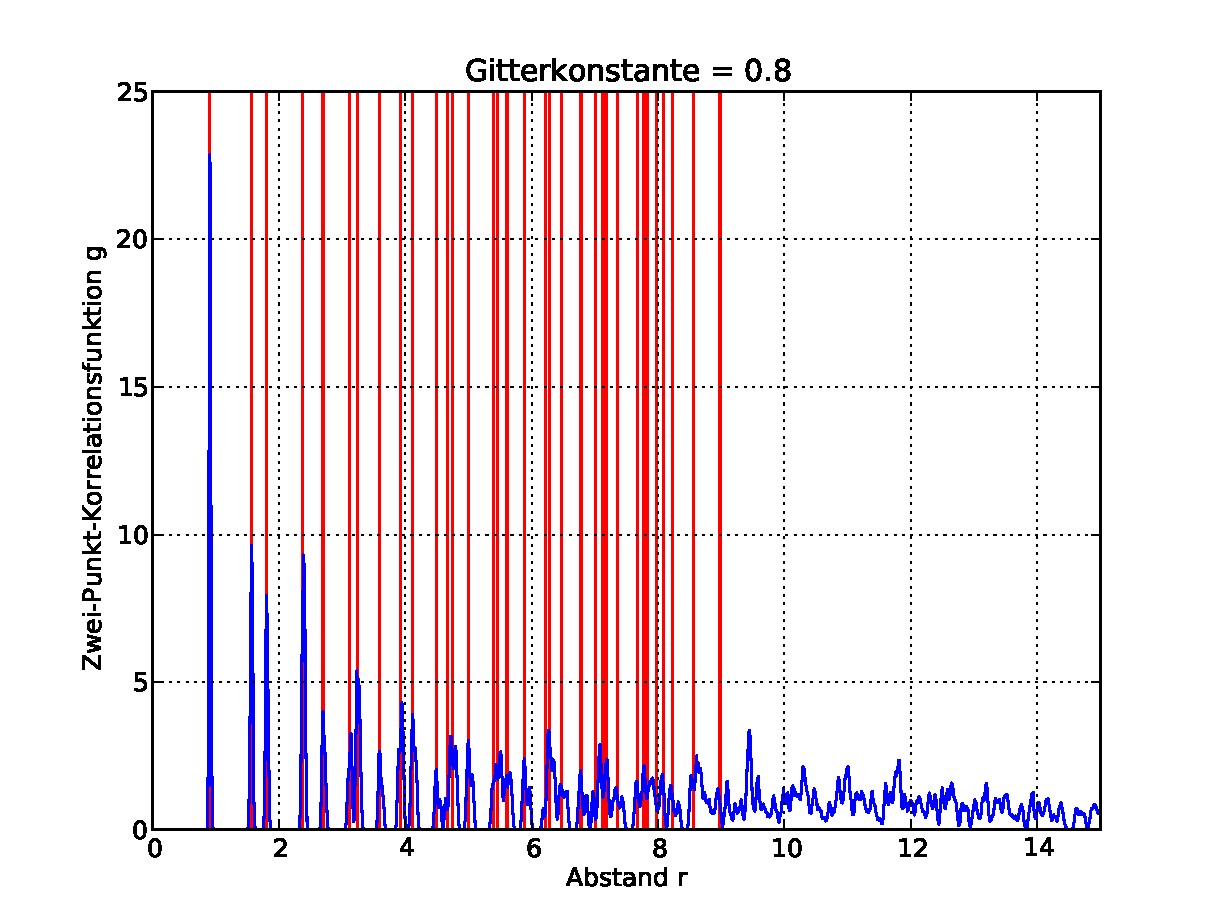
\includegraphics[width=0.70\textwidth]{img/Korr08.pdf}
	\caption{Korrelation f�r eine Gitterkonstante von $0.8r_c$. Der erste Peak liegt bei $0.90$}
	\label{fig:Korr08}
\end{figure}
\begin{figure}[h!]
	\centering
		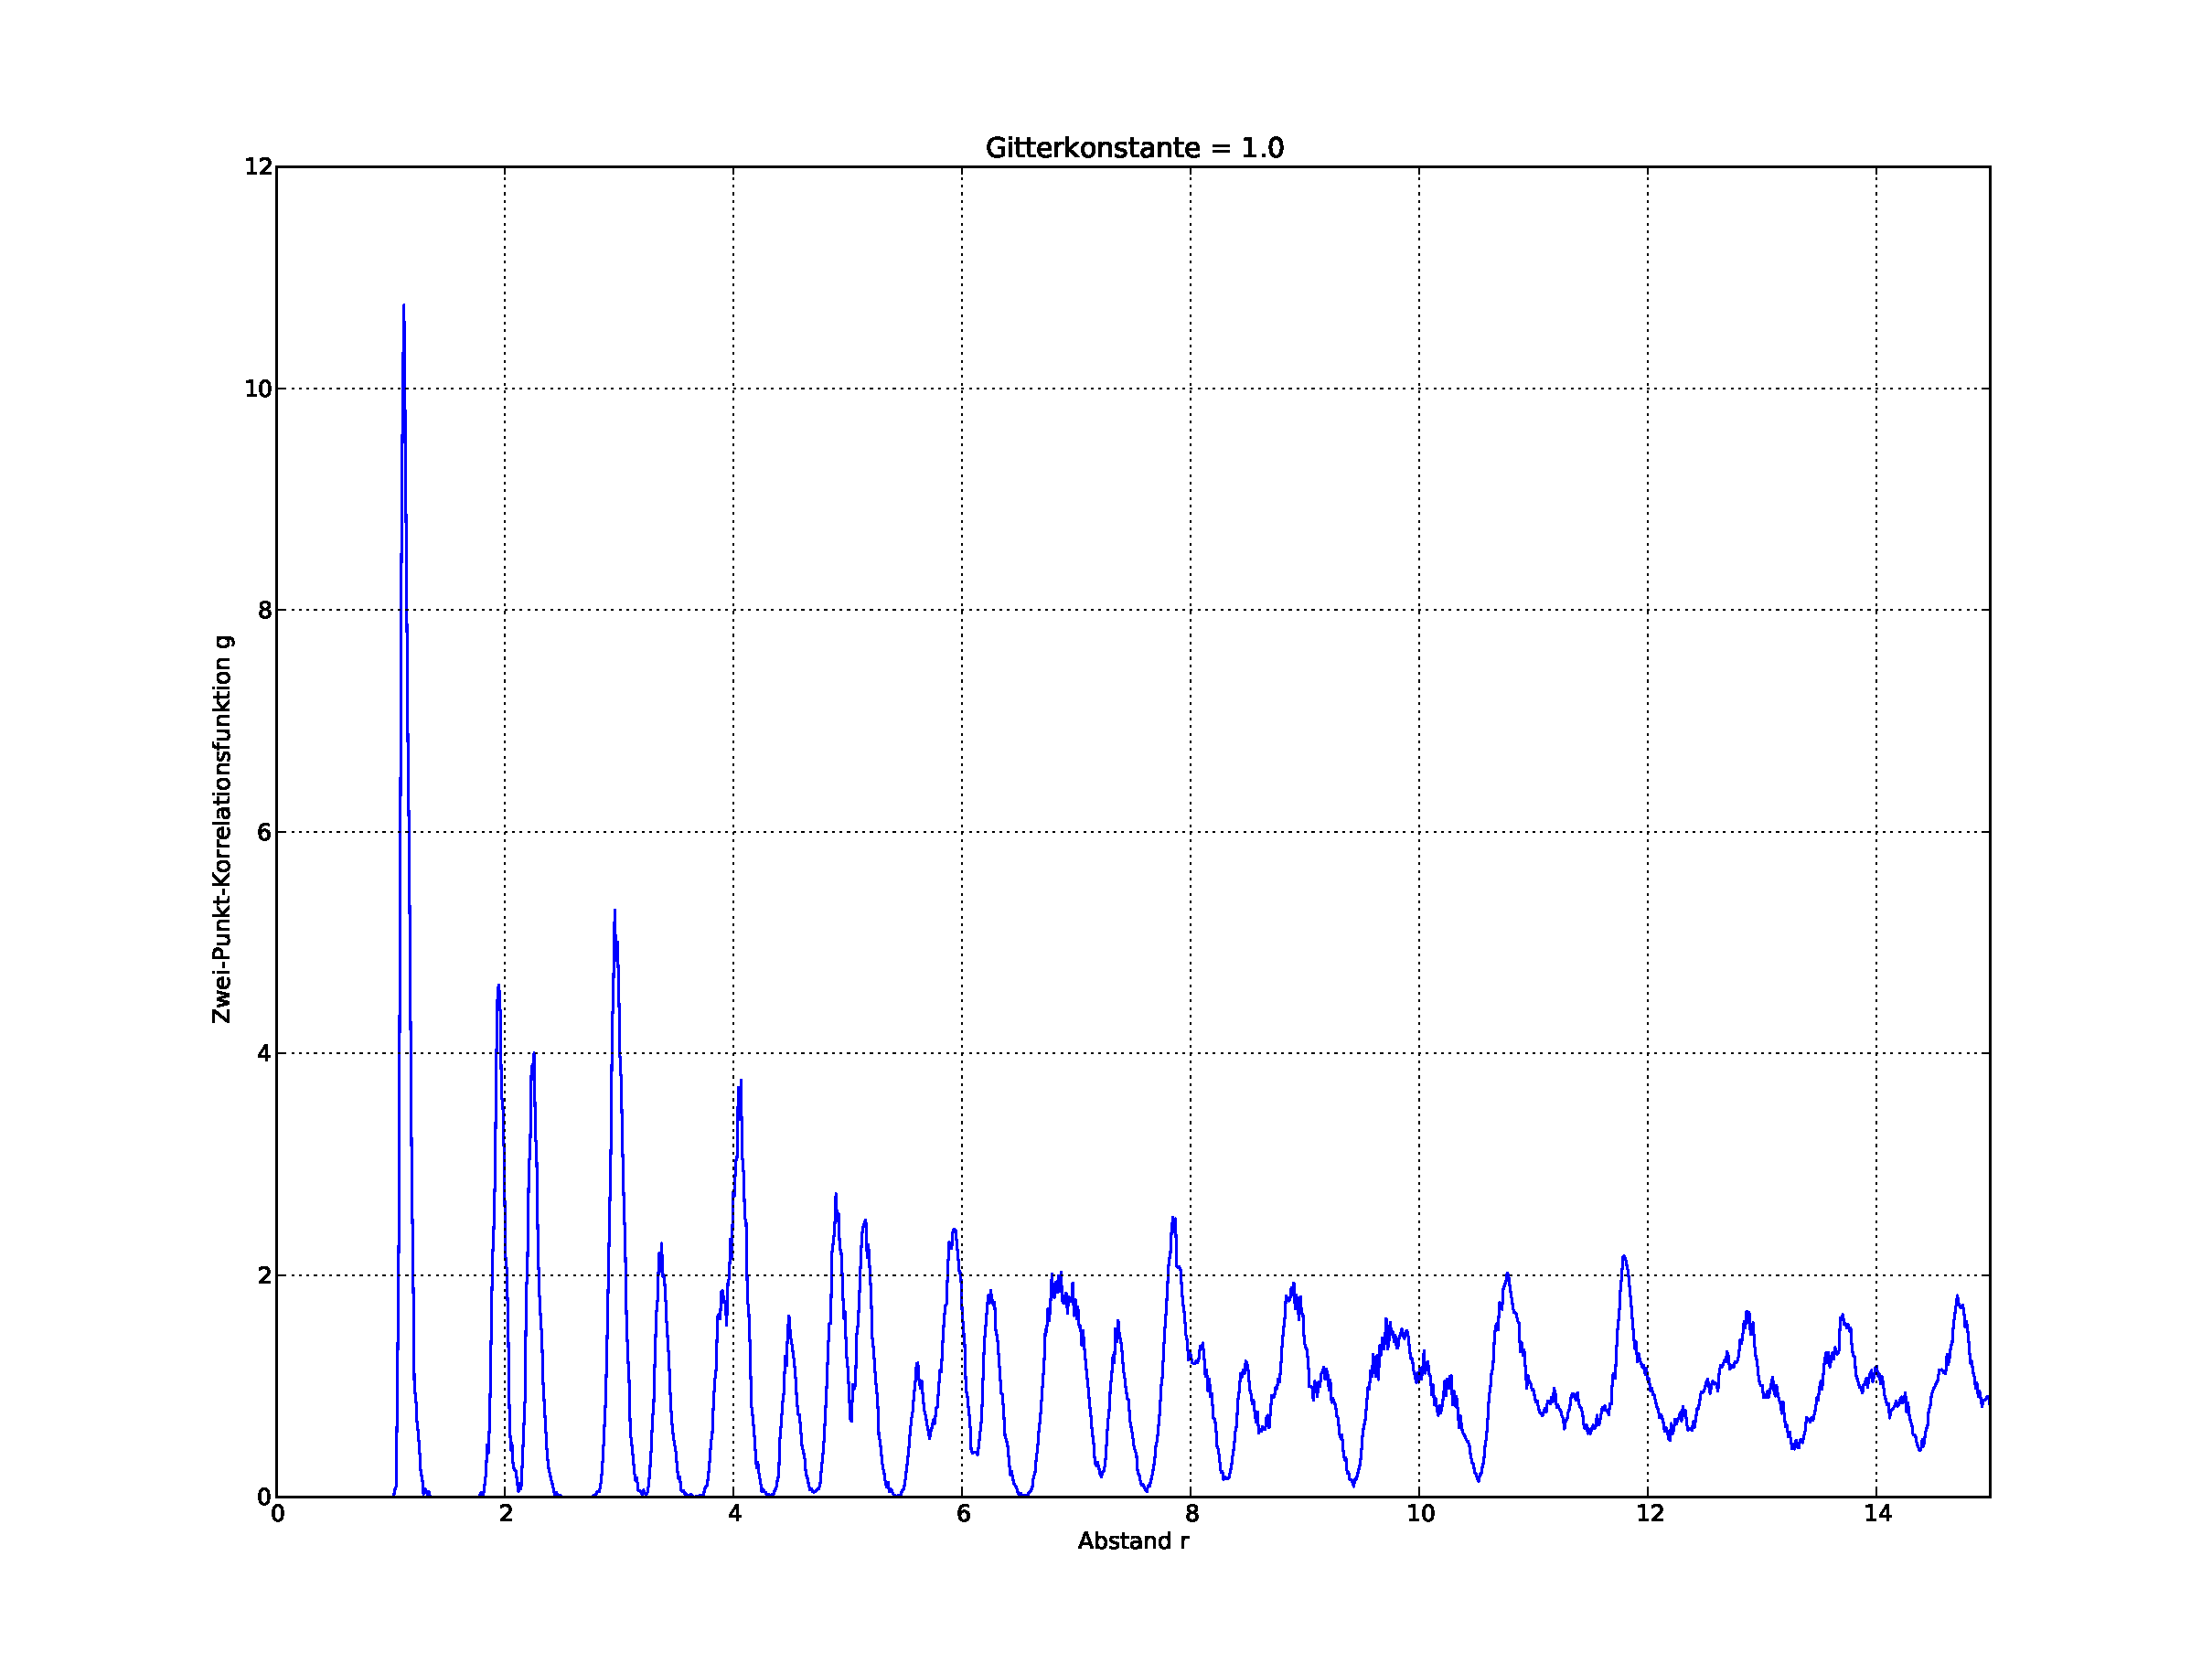
\includegraphics[width=0.70\textwidth]{img/Korr1.pdf}
	\caption{Korrelation f�r eine Gitterkonstante von $1.0r_c$. Der erste Peak liegt bei $1.12$}
	\label{fig:Korr1}
\end{figure}
\begin{figure}[h!]
	\centering
		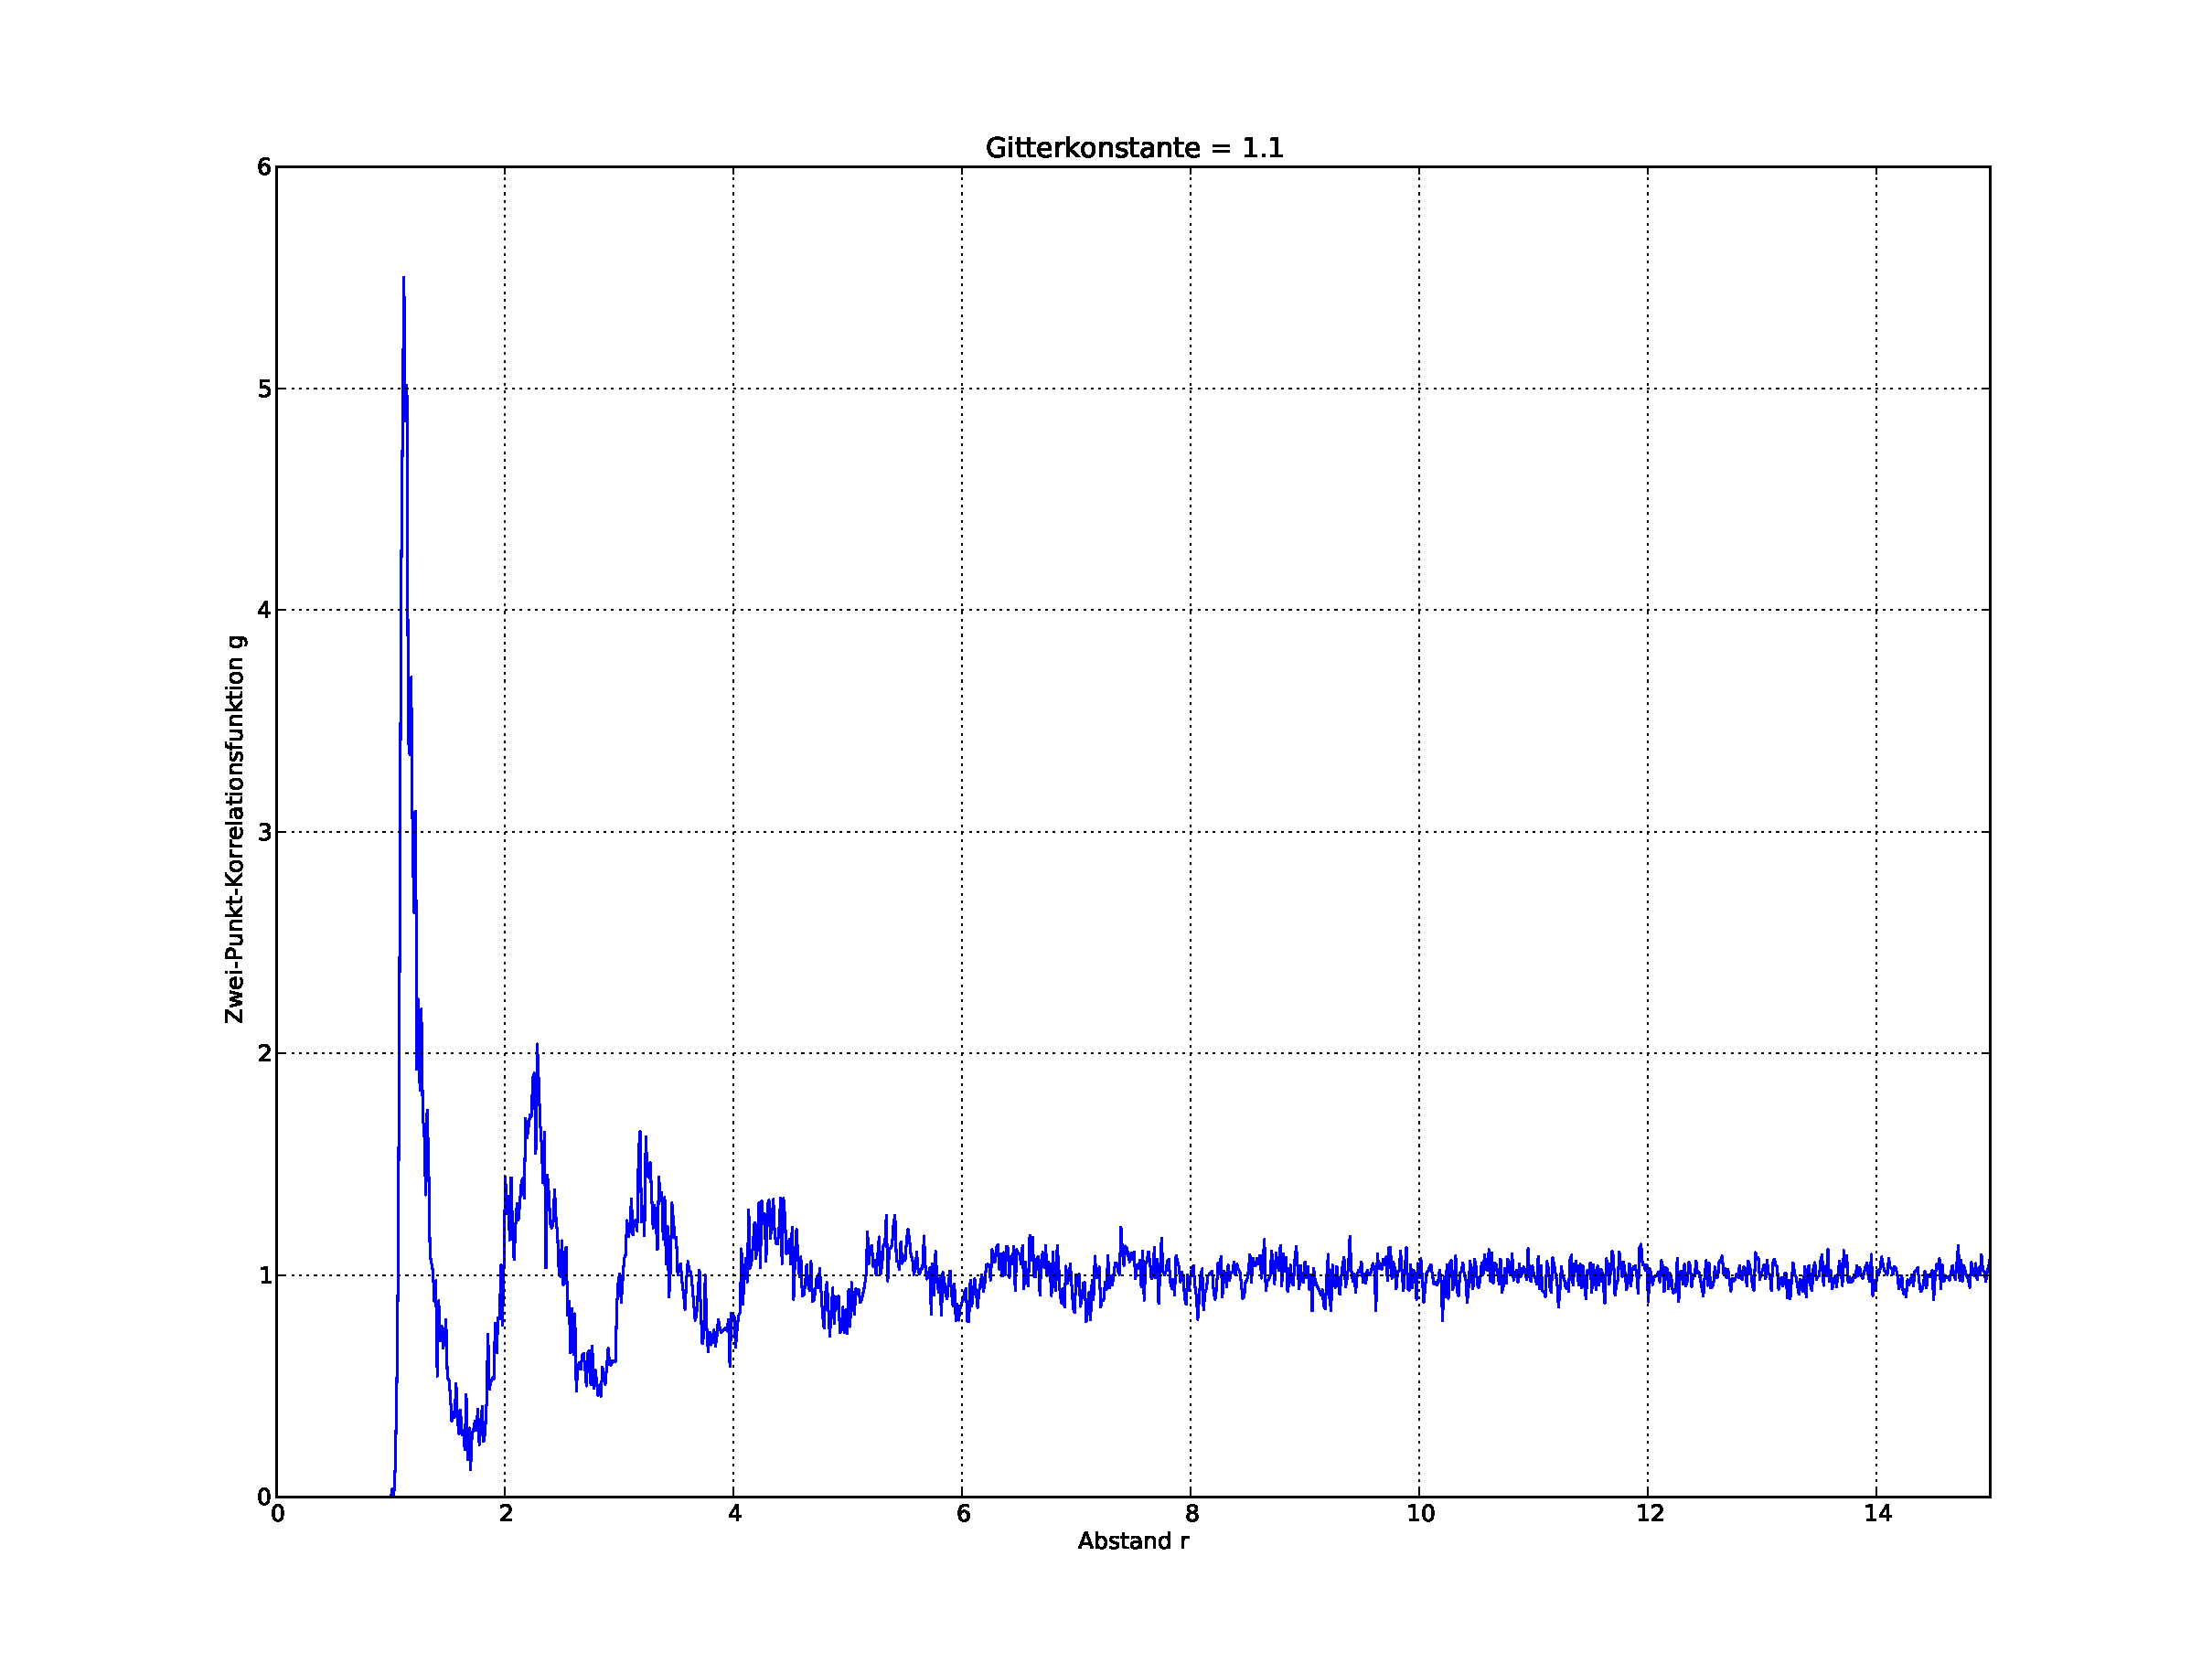
\includegraphics[width=0.70\textwidth]{img/Korr11.pdf}
	\caption{Korrelation f�r eine Gitterkonstante von $1.1r_c$. Der erste Peak liegt bei $1.12$}
	\label{fig:Korr11}
\end{figure}
\begin{figure}[h!]
	\centering
		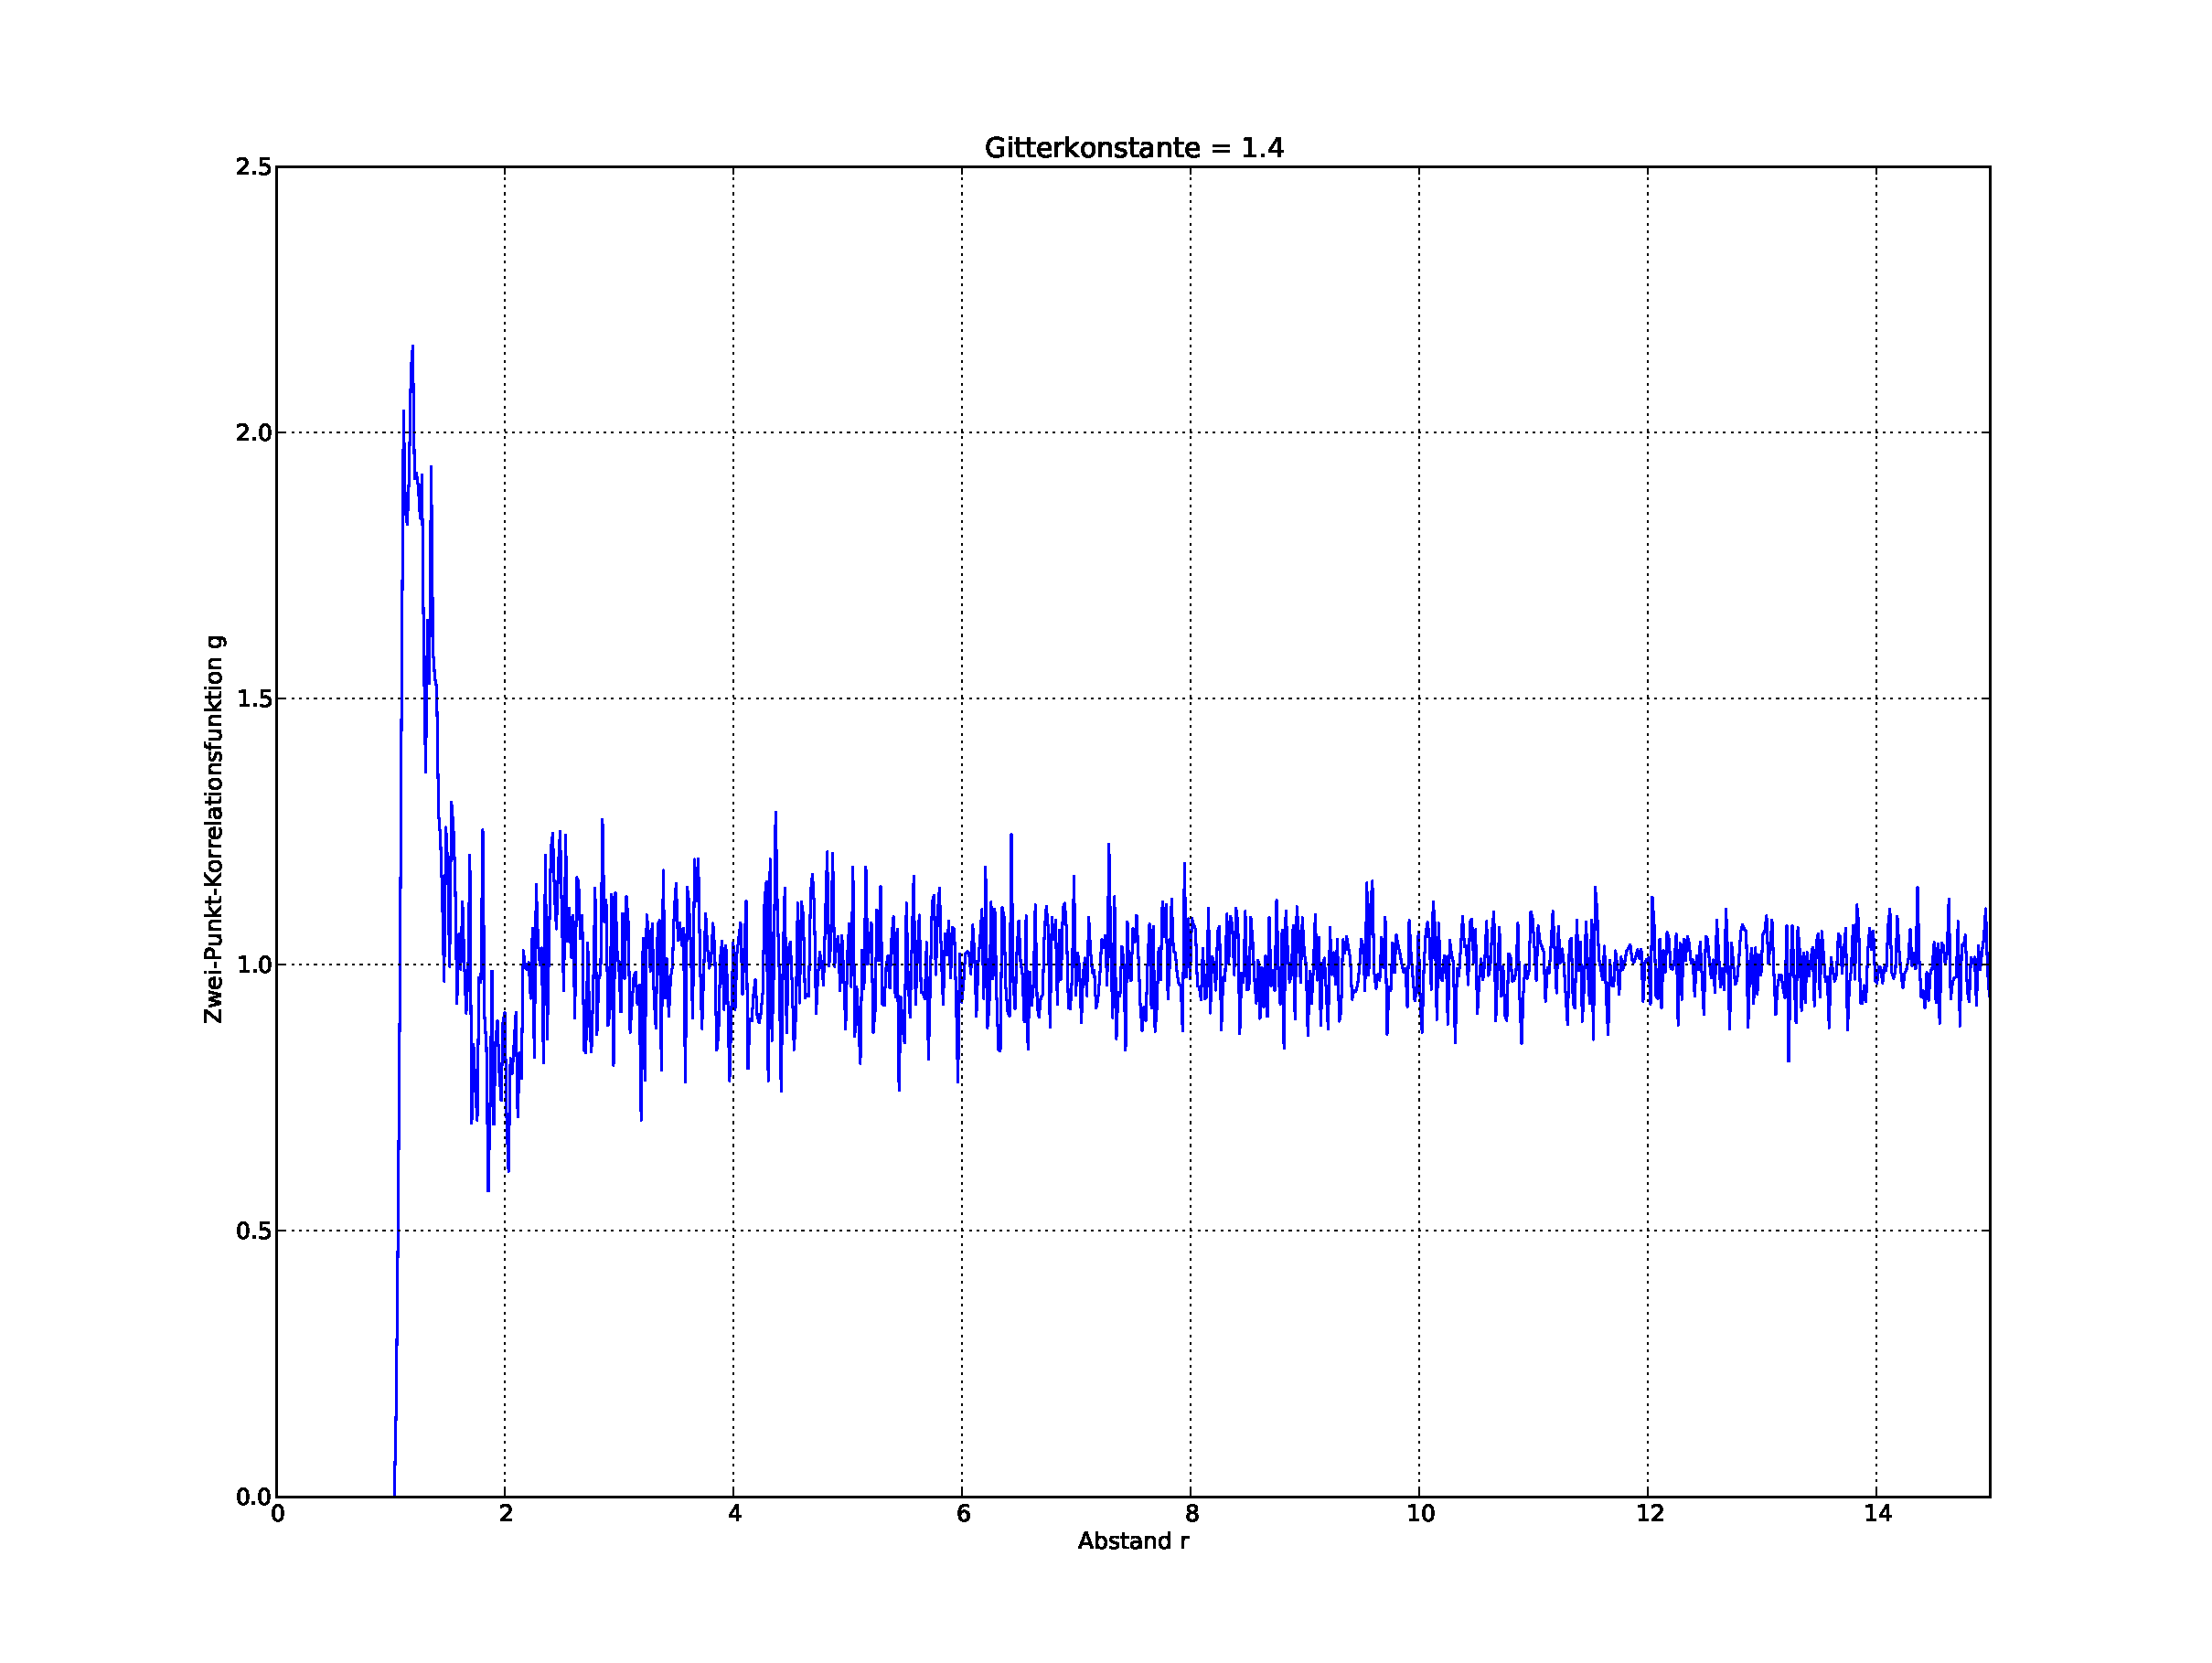
\includegraphics[width=0.70\textwidth]{img/Korr14.pdf}
	\caption{Korrelation f�r eine Gitterkonstante von $1.4r_c$. Der erste Peak liegt bei $1.12$}
	\label{fig:Korr14}
\end{figure}

